\chapter{Lewis Structures and the Shape of Molecules}\label{ch:g10:lewis-and-shape}

A \omterm{def:g7:atoms-and-molecules:molecule}{molecule} of carbon dioxide is straight; a \omterm{def:g7:atoms-and-molecules:molecule}{molecule} of water is bent.
That single difference in shape is one of the reasons why water, with
\omterm{def:g7:atoms-and-molecules:molecule}{molecules} lighter than those of carbon dioxide, is a liquid at room
temperature while carbon dioxide is a gas. \omterm{def:g7:atoms-and-molecules:atom}{Atoms} in a \omterm{def:g7:atoms-and-molecules:molecule}{molecule} are held
together by shared \omterm{def:g9:inside-the-atom:nucleus}{electrons}, and the way the \omterm{def:g9:inside-the-atom:nucleus}{electrons} are shared
decides the shape. This chapter draws the shared \omterm{def:g9:inside-the-atom:nucleus}{electrons}, and from
them predicts the shape.

\begin{recall}
The \omterm{def:g10:electron-shells:valence}{valence electrons} are those of the outer \omterm{def:g10:electron-shells:configuration}{shell}; \omterm{def:g7:atoms-and-molecules:atom}{atoms} tend to reach
the configuration of a \omterm{def:g10:electron-shells:family}{noble gas}, eight \omterm{def:g9:inside-the-atom:nucleus}{electrons} in the outer \omterm{def:g10:electron-shells:configuration}{shell}
(\omterm{def:g10:electron-shells:octet}{octet rule}) or two for hydrogen (\omterm{def:g10:electron-shells:octet}{duet rule})
(\cref{ch:g10:electron-shells}). Molecular models show \omterm{def:g7:atoms-and-molecules:atom}{atoms} as balls and
bonds as sticks (\cref{ch:g7:atoms-and-molecules}).
\end{recall}

\section{The covalent bond}

\begin{definition}[Covalent bond]\label{def:g10:lewis-and-shape:covalent-bond}
A \emph{covalent bond}\index{covalent bond} is a pair of \omterm{def:g9:inside-the-atom:nucleus}{electrons} shared
by two \omterm{def:g7:atoms-and-molecules:atom}{atoms}; each \omterm{def:g7:atoms-and-molecules:atom}{atom} usually provides one \omterm{def:g9:inside-the-atom:nucleus}{electron} of the pair. Both
\omterm{def:g7:atoms-and-molecules:atom}{atoms} count the shared pair in their outer \omterm{def:g10:electron-shells:configuration}{shell}, which lets both reach
a duet or an octet.
\end{definition}

\begin{definition}[Bonding pairs and lone pairs]\label{def:g10:lewis-and-shape:lone-pair}
In a \omterm{def:g7:atoms-and-molecules:molecule}{molecule}, the \omterm{def:g10:electron-shells:valence}{valence electrons} of each \omterm{def:g7:atoms-and-molecules:atom}{atom} are grouped in pairs.
A \emph{bonding pair}\index{bonding pair} is shared between two \omterm{def:g7:atoms-and-molecules:atom}{atoms} and
forms a \omterm{def:g10:lewis-and-shape:covalent-bond}{covalent bond}; a \emph{lone pair}\index{lone pair} belongs to a
single \omterm{def:g7:atoms-and-molecules:atom}{atom} and takes no part in a bond.
\end{definition}

\begin{proposition}[How many bonds an atom forms]\label{prop:g10:lewis-and-shape:valence}
An \omterm{def:g7:atoms-and-molecules:atom}{atom} forms as many \omterm{def:g10:lewis-and-shape:covalent-bond}{covalent bonds} as it lacks \omterm{def:g9:inside-the-atom:nucleus}{electrons} to complete its
duet or octet:
\begin{center}
\small
\begin{tabular}{lcccc}
\hline
\omterm{def:g7:atoms-and-molecules:atom}{atom} & \omterm{def:g10:electron-shells:valence}{valence electrons} & bonds & \omterm{def:g10:lewis-and-shape:lone-pair}{lone pairs} & example \\
\hline
H & 1 & 1 & 0 & \ce{H2} \\
C & 4 & 4 & 0 & \ce{CH4} \\
N & 5 & 3 & 1 & \ce{NH3} \\
O & 6 & 2 & 2 & \ce{H2O} \\
Cl & 7 & 1 & 3 & \ce{HCl} \\
\hline
\end{tabular}
\end{center}
\end{proposition}

\section{Lewis structures}

\begin{definition}[Lewis structure]\label{def:g10:lewis-and-shape:lewis-structure}
The \emph{Lewis structure}\index{Lewis structure} of a \omterm{def:g7:atoms-and-molecules:molecule}{molecule} shows
its \omterm{def:g7:atoms-and-molecules:atom}{atoms} by their symbols, each \omterm{def:g10:lewis-and-shape:lone-pair}{bonding pair} by a line between two \omterm{def:g7:atoms-and-molecules:atom}{atoms}
and each \omterm{def:g10:lewis-and-shape:lone-pair}{lone pair} by a pair of dots next to its \omterm{def:g7:atoms-and-molecules:atom}{atom}.
\end{definition}

\begin{definition}[Double and triple bonds]\label{def:g10:lewis-and-shape:multiple-bond}
Two \omterm{def:g7:atoms-and-molecules:atom}{atoms} may share two pairs of \omterm{def:g9:inside-the-atom:nucleus}{electrons}, a \emph{double
bond}\index{double bond}, drawn as two lines, or three pairs, a
\emph{triple bond}\index{triple bond}, drawn as three lines.
\end{definition}

\begin{method}[Drawing a Lewis structure]\label{met:g10:lewis-and-shape:draw}
\begin{enumerate}
  \item Add up the \omterm{def:g10:electron-shells:valence}{valence electrons} of all the \omterm{def:g7:atoms-and-molecules:atom}{atoms}, and halve to get
        the number of pairs.
  \item Join the \omterm{def:g7:atoms-and-molecules:atom}{atoms} by single bonds (hydrogen, which forms one bond,
        is always on the outside; carbon is usually central).
  \item Place the remaining pairs as \omterm{def:g10:lewis-and-shape:lone-pair}{lone pairs}, first on the outer \omterm{def:g7:atoms-and-molecules:atom}{atoms},
        to complete their octets.
  \item If an \omterm{def:g7:atoms-and-molecules:atom}{atom} still lacks an octet, turn a \omterm{def:g10:lewis-and-shape:lone-pair}{lone pair} of a neighbour
        into a second (or third) shared pair.
  \item Check: every hydrogen has 2 \omterm{def:g9:inside-the-atom:nucleus}{electrons}, every other \omterm{def:g7:atoms-and-molecules:atom}{atom} 8, and
        all the pairs have been used.
\end{enumerate}
\end{method}

\begin{example}[Carbon dioxide]\label{ex:g10:lewis-and-shape:co2}
\ce{CO2}: $4 + 2 \times 6 = 16$ \omterm{def:g10:electron-shells:valence}{valence electrons}, 8 pairs. Single bonds
\ce{O-C-O} use 2 pairs; 6 \omterm{def:g10:lewis-and-shape:lone-pair}{lone pairs} on the oxygens complete them, but
carbon then has only 4 \omterm{def:g9:inside-the-atom:nucleus}{electrons}. Turning one \omterm{def:g10:lewis-and-shape:lone-pair}{lone pair} of each oxygen
into a shared pair gives two \omterm{def:g10:lewis-and-shape:multiple-bond}{double bonds}: each \omterm{def:g7:atoms-and-molecules:atom}{atom} now has an octet.
\end{example}

\begin{omfigure}
\setchemfig{atom sep=2.0em}
\begin{tabular}{cccccc}
\chemfig{H-H} & \chemfig{H-\charge{0=\:,90=\:,270=\:}{Cl}} & \chemfig{H-\charge{90=\:,270=\:}{O}-H} &
\chemfig{H-\charge{90=\:}{N}(-[6]H)-H} & \chemfig{H-C(-[2]H)(-[6]H)-H} &
\chemfig{\charge{135=\:,225=\:}{O}=C=\charge{45=\:,315=\:}{O}} \\[4pt]
\small \ce{H2} & \small \ce{HCl} & \small \ce{H2O} & \small \ce{NH3} & \small \ce{CH4} & \small \ce{CO2} \\[10pt]
\chemfig{\charge{180=\:}{N}~\charge{0=\:}{N}} & \chemfig{\charge{135=\:,225=\:}{O}=\charge{45=\:,315=\:}{O}} &
\chemfig{C(-[3]H)(-[5]H)=C(-[1]H)-[7]H} & \chemfig{H-C~\charge{0=\:}{N}} &
\chemfig{H-C(-[6]H)=\charge{45=\:,315=\:}{O}} & \\[4pt]
\small \ce{N2} & \small \ce{O2} & \small \ce{C2H4} & \small \ce{HCN} & \small methanal \ce{CH2O} &
\end{tabular}

{\small \omterm{def:g10:lewis-and-shape:lewis-structure}{Lewis structures} of eleven \omterm{def:g7:atoms-and-molecules:molecule}{molecules}. Every \omterm{def:g7:atoms-and-molecules:atom}{atom} other than
hydrogen is surrounded by four pairs (bonds and \omterm{def:g10:lewis-and-shape:lone-pair}{lone pairs}): an octet.}
\end{omfigure}

\section{The shape of molecules}

\begin{proposition}[Electron pairs keep as far apart as possible]\label{prop:g10:lewis-and-shape:shape}
Around a central \omterm{def:g7:atoms-and-molecules:atom}{atom}, the groups of \omterm{def:g9:inside-the-atom:nucleus}{electrons} --- each single, double or
\omterm{def:g10:lewis-and-shape:multiple-bond}{triple bond}, and each \omterm{def:g10:lewis-and-shape:lone-pair}{lone pair} --- repel one another and settle as far
apart as possible. The shape of the \omterm{def:g7:atoms-and-molecules:molecule}{molecule} follows:
\begin{center}
\small
\begin{tabular}{llll}
\hline
groups around the centre & of which \omterm{def:g10:lewis-and-shape:lone-pair}{lone pairs} & shape & example \\
\hline
2 & 0 & linear, angle \ang{180} & \ce{CO2}, \ce{HCN} \\
3 & 0 & flat triangle, angle \ang{120} & \ce{CH2O}, \ce{C2H4} \\
4 & 0 & tetrahedron, angle \ang{109.5} & \ce{CH4} \\
4 & 1 & pyramid & \ce{NH3} \\
4 & 2 & bent & \ce{H2O} \\
\hline
\end{tabular}
\end{center}
\end{proposition}
\admitted

\begin{remark}[Where this comes from]\label{rem:g10:lewis-and-shape:vsepr}
This rule is a model, and it works remarkably well for small \omterm{def:g7:atoms-and-molecules:molecule}{molecules};
it is made precise, and partly explained, in the Year 1 volume. \omterm{def:g10:lewis-and-shape:lone-pair}{Lone pairs}
take up a little more room than \omterm{def:g10:lewis-and-shape:lone-pair}{bonding pairs}: the angle in ammonia
(\ang{106.7}) and in water (\ang{104.5}) is a little smaller than the
\ang{109.5} of methane.
\end{remark}

\begin{omfigure}
\begin{tikzpicture}[font=\small]
  % methane, tetrahedral, in perspective
  \begin{scope}
    \node[aC] (c) at (0,0) {};
    \node[aH, minimum size=3.6mm] (hb) at (0.3,-0.12) {};
    \node[aH] (h1) at (0,1.05) {};
    \node[aH] (h2) at (-1.0,-0.45) {};
    \node[aH] (h3) at (0.72,-0.5) {};
    \begin{scope}[on background layer]
      \foreach \h in {h1,h2,h3,hb} \draw[bond] (c.center) -- (\h.center);
    \end{scope}
    \node[aC] at (0,0) {};
    \node at (0,-1.35) {methane: tetrahedron};
    \node[font=\footnotesize] at (-0.55,0.55) {\ang{109.5}};
  \end{scope}
  % ammonia, pyramid
  \begin{scope}[xshift=4.2cm]
    \fill[omDef!25] (0,0.2) ellipse (0.18 and 0.45);
    \node[font=\scriptsize, omDef] at (0,1.0) {lone pair};
    \node[aN] (n) at (0,0) {};
    \node[aH] (h1) at (-0.95,-0.5) {};
    \node[aH] (h2) at (0.7,-0.55) {};
    \node[aH, minimum size=3.6mm] (h3) at (0.25,-0.2) {};
    \begin{scope}[on background layer]
      \foreach \h in {h1,h2,h3} \draw[bond] (n.center) -- (\h.center);
    \end{scope}
    \node[aN] at (0,0) {};
    \node at (0,-1.35) {ammonia: pyramid};
  \end{scope}
  % water, bent
  \begin{scope}[xshift=8.4cm]
    \fill[omDef!25, rotate=25] (0,0.2) ellipse (0.16 and 0.42);
    \fill[omDef!25, rotate=-25] (0,0.2) ellipse (0.16 and 0.42);
    \node[aO] (o) at (0,0) {};
    \node[aH] (h1) at (-0.8,-0.58) {};
    \node[aH] (h2) at (0.8,-0.58) {};
    \begin{scope}[on background layer]
      \draw[bond] (o.center) -- (h1.center); \draw[bond] (o.center) -- (h2.center);
    \end{scope}
    \node[aO] at (0,0) {};
    \draw[black!60] (-0.32,-0.23) arc[start angle=216, end angle=324, radius=0.4];
    \node[font=\footnotesize] at (0,-0.65) {\ang{104.5}};
    \node at (0,-1.35) {water: bent};
  \end{scope}
  % carbon dioxide, linear
  \begin{scope}[xshift=12.0cm]
    \node[aO] (a) at (-0.8,0) {}; \node[aC] (c) at (0,0) {}; \node[aO] (b) at (0.8,0) {};
    \begin{scope}[on background layer]
      \foreach \d in {-1.6,1.6} {
        \draw[bond, line width=1.1pt] ([yshift=\d pt]a.center) -- ([yshift=\d pt]c.center);
        \draw[bond, line width=1.1pt] ([yshift=\d pt]c.center) -- ([yshift=\d pt]b.center);}
    \end{scope}
    \node at (0,-1.35) {carbon dioxide: linear};
  \end{scope}
\end{tikzpicture}

{\small Shapes of four \omterm{def:g7:atoms-and-molecules:molecule}{molecules} (\omterm{def:g10:lewis-and-shape:lone-pair}{lone pairs} shown as shaded lobes).
% ledger: ang:H2O, ang:NH3
Methane is a tetrahedron, ammonia a pyramid, water bent, carbon dioxide
straight.}
\end{omfigure}

\begin{omfigure}
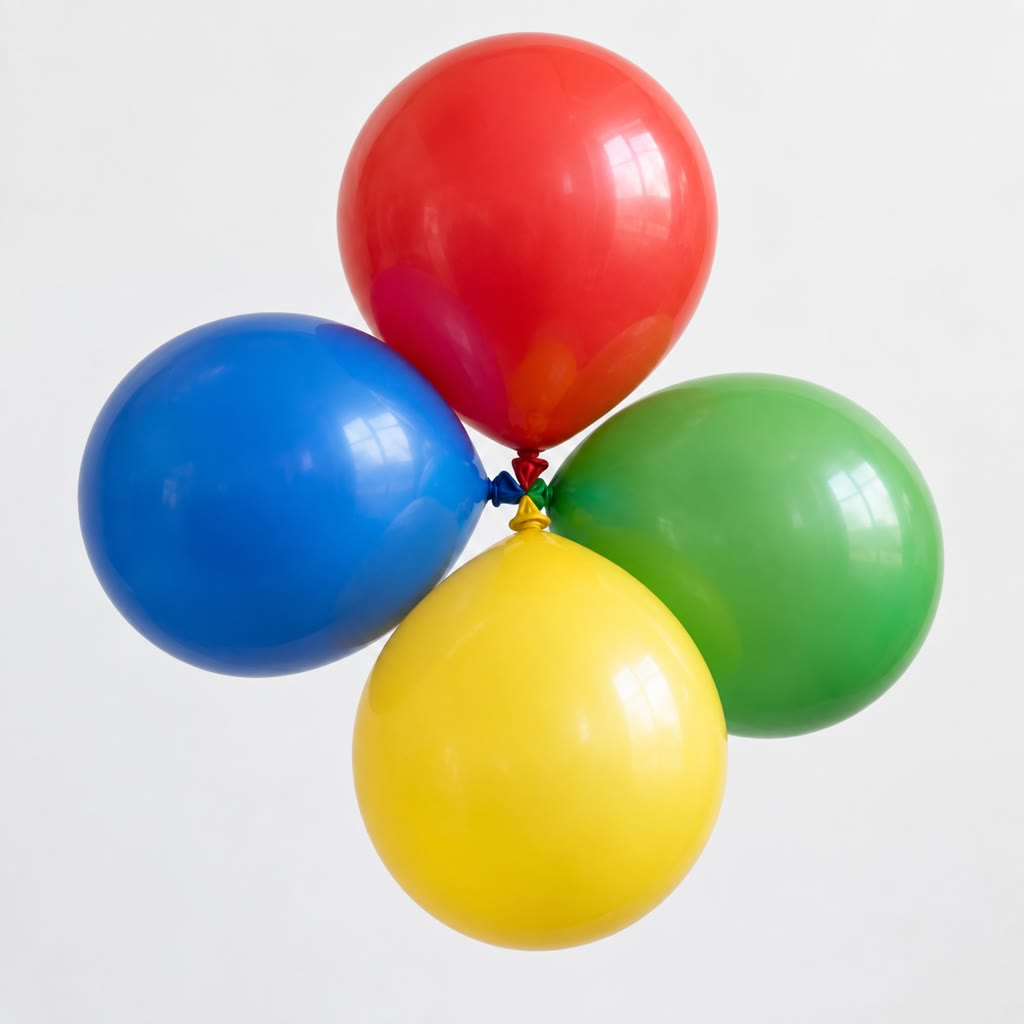
\includegraphics[width=0.38\linewidth]{images/book1/ai/g10-balloons-tetrahedron.jpg}

{\small Four balloons tied together push one another as far apart as they
can; in space they point to the corners of a tetrahedron, like the four
\omterm{def:g9:inside-the-atom:nucleus}{electron} pairs around a carbon \omterm{def:g7:atoms-and-molecules:atom}{atom}.}
\end{omfigure}

\section{Drawing molecules in space}

\begin{notation}[Wedges and dashes]\label{not:g10:lewis-and-shape:wedge}
To draw a \omterm{def:g7:atoms-and-molecules:molecule}{molecule} in space on flat paper, a bond in the plane of the
paper is a plain line, a bond pointing towards the reader a solid wedge,
and a bond pointing away a dashed wedge. Methane is then drawn as below:
two bonds in the plane, one towards and one away from the reader.
\begin{center}
\chemfig{C(-[2]H)(-[4]H)(<[7]H)(<:[5]H)}
\end{center}
\end{notation}

\section{Exercises}

\begin{exercise}[$\star$]\label{exo:g10:lewis-and-shape:1}
What is a \omterm{def:g10:lewis-and-shape:covalent-bond}{covalent bond}? What is a \omterm{def:g10:lewis-and-shape:lone-pair}{lone pair}?
\end{exercise}

\begin{exercise}[$\star$]\label{exo:g10:lewis-and-shape:2}
How many \omterm{def:g10:lewis-and-shape:covalent-bond}{covalent bonds} do hydrogen, carbon, nitrogen and oxygen usually
form? Explain with the octet and \omterm{def:g10:electron-shells:octet}{duet rules}.
\end{exercise}

\begin{exercise}[$\star$]\label{exo:g10:lewis-and-shape:3}
Draw the \omterm{def:g10:lewis-and-shape:lewis-structure}{Lewis structure} of hydrogen chloride, \ce{HCl}, and count the
\omterm{def:g9:inside-the-atom:nucleus}{electrons} around chlorine.
\end{exercise}

\begin{exercise}[$\star$]\label{exo:g10:lewis-and-shape:4}
How many \omterm{def:g10:electron-shells:valence}{valence electrons}, in all, does the \omterm{def:g7:atoms-and-molecules:molecule}{molecule} \ce{NH3} have? How
many pairs?
\end{exercise}

\begin{exercise}[$\star$]\label{exo:g10:lewis-and-shape:5}
Give the shape of \ce{CH4}, \ce{NH3}, \ce{H2O} and \ce{CO2}.
\end{exercise}

\begin{exercise}[$\star\star$]\label{exo:g10:lewis-and-shape:6}
Draw the \omterm{def:g10:lewis-and-shape:lewis-structure}{Lewis structure} of hydrogen sulfide, \ce{H2S} (sulfur is in the
group of oxygen), and predict its shape.
\end{exercise}

\begin{exercise}[$\star\star$]\label{exo:g10:lewis-and-shape:7}
Draw the \omterm{def:g10:lewis-and-shape:lewis-structure}{Lewis structure} of nitrogen, \ce{N2}, following the method step by
step.
\end{exercise}

\begin{exercise}[$\star\star$]\label{exo:g10:lewis-and-shape:8}
Draw the \omterm{def:g10:lewis-and-shape:lewis-structure}{Lewis structure} of methanol, \ce{CH3OH}, and give the shape
around the carbon and around the oxygen.
\end{exercise}

\begin{exercise}[$\star\star$]\label{exo:g10:lewis-and-shape:9}
Why is \ce{CO2} linear and \ce{H2O} bent, although both have a central \omterm{def:g7:atoms-and-molecules:atom}{atom}
joined to two others?
\end{exercise}

\begin{exercise}[$\star\star$]\label{exo:g10:lewis-and-shape:10}
Draw the \omterm{def:g10:lewis-and-shape:lewis-structure}{Lewis structure} of ethene, \ce{C2H4}, and give the shape around
each carbon \omterm{def:g7:atoms-and-molecules:atom}{atom}.
\end{exercise}

\begin{exercise}[$\star\star$]\label{exo:g10:lewis-and-shape:11}
Draw the \omterm{def:g10:lewis-and-shape:lewis-structure}{Lewis structure} of tetrachloromethane, \ce{CCl4}, and predict its
shape.
\end{exercise}

\begin{exercise}[$\star\star\star$]\label{exo:g10:lewis-and-shape:12}
Two \omterm{def:g7:atoms-and-molecules:molecule}{molecules} have the formula \ce{C2H6O}. Draw a \omterm{def:g10:lewis-and-shape:lewis-structure}{Lewis structure} for each
(one has an O--H bond, the other a C--O--C chain).
\end{exercise}

\begin{exercise}[$\star\star\star$]\label{exo:g10:lewis-and-shape:13}
Explain, using \omterm{def:g10:lewis-and-shape:lone-pair}{lone pairs}, why the angle in ammonia (\ang{106.7}) is
smaller than in methane (\ang{109.5}), and in water (\ang{104.5}) smaller
still.
\end{exercise}

\begin{exercise}[$\star\star\star$]\label{exo:g10:lewis-and-shape:14}
Draw the \omterm{def:g10:lewis-and-shape:lewis-structure}{Lewis structure} of hydrogen cyanide, \ce{HCN}, and of methanal,
\ce{CH2O}, and give their shapes.
\end{exercise}

\begin{exercise}[$\star\star\star$]\label{exo:g10:lewis-and-shape:15}
Ozone, \ce{O3}, is a chain of three oxygen \omterm{def:g7:atoms-and-molecules:atom}{atoms}. Count its valence pairs
and draw a \omterm{def:g10:lewis-and-shape:lewis-structure}{Lewis structure} in which every oxygen has an octet (one
\omterm{def:g10:lewis-and-shape:multiple-bond}{double bond}, one single bond). Predict whether the \omterm{def:g7:atoms-and-molecules:molecule}{molecule} is linear or
bent.
\end{exercise}

\section{Problem: A Molecule in a Cube}

\begin{problem}[{Weekend problem --- designing the carbon balls of a
molecular model kit: at what angle must the holes be drilled?}]
\label{pb:g10:lewis-and-shape:1}
% ledger: ang:H2O, ang:NH3
A company makes molecular model kits. The black carbon balls must have
four holes, so that methane, ethane and the other \omterm{def:g7:atoms-and-molecules:molecule}{molecules} of carbon come
out with the right shape. The engineer uses a trick: a regular
tetrahedron fits inside a cube, its four corners on four corners of the
cube, none two on the same edge.

\medskip
\noindent\textbf{Part I --- \omterm{def:g10:lewis-and-shape:lewis-structure}{Lewis structures}.}
\begin{enumerate}
  \item Draw the \omterm{def:g10:lewis-and-shape:lewis-structure}{Lewis structures} of methane \ce{CH4}, ammonia \ce{NH3} and
        water \ce{H2O}.
  \item How many groups of \omterm{def:g9:inside-the-atom:nucleus}{electrons} surround the central \omterm{def:g7:atoms-and-molecules:atom}{atom} in each?
  \item How many of them are \omterm{def:g10:lewis-and-shape:lone-pair}{lone pairs}?
  \item Why does a carbon ball need four holes, and an oxygen ball (for
        water) only two?
  \item A model of ethane, \ce{C2H6}, uses two carbon balls. Draw its \omterm{def:g10:lewis-and-shape:lewis-structure}{Lewis
        structure}. How many sticks join the two carbon balls, and how many
        hydrogen balls are needed?
\end{enumerate}

\medskip
\noindent\textbf{Part II --- Shapes.}
\begin{enumerate}[resume]
  \item Give the shape of each of the three \omterm{def:g7:atoms-and-molecules:molecule}{molecules}.
  \item The measured angles are \ang{106.7} in ammonia and \ang{104.5} in
        water. Explain why they are smaller than the angle of methane.
  \item Why can the oxygen ball for water not simply be a carbon ball with
        two holes left empty, if the kit is to show the true angle?
  \item In carbon dioxide, the carbon \omterm{def:g7:atoms-and-molecules:atom}{atom} forms two \omterm{def:g10:lewis-and-shape:multiple-bond}{double bonds}. Which
        angle must separate them in a model?
\end{enumerate}

\medskip
\noindent\textbf{Part III --- The cube.}
Take a cube of side $a$. The carbon \omterm{def:g7:atoms-and-molecules:atom}{atom} is at its centre; the four
hydrogen \omterm{def:g7:atoms-and-molecules:atom}{atoms} sit on four corners of the cube, none two on the same edge.
\begin{enumerate}[resume]
  \item Show that any two of these hydrogen \omterm{def:g7:atoms-and-molecules:atom}{atoms} are at the two ends of
        a diagonal of a face of the cube. Using Pythagoras, compute the
        distance between them in terms of $a$.
  \item The diagonal of the whole cube (from a corner to the opposite
        corner) has length $a\sqrt{3}$. Deduce the distance from the
        carbon \omterm{def:g7:atoms-and-molecules:atom}{atom} to a hydrogen \omterm{def:g7:atoms-and-molecules:atom}{atom}.
  \item Take $a = \qty{1}{cm}$ in a model: give both distances in
        centimetres, to two decimal places.
  \item Why are the four C--H distances equal?
\end{enumerate}

\medskip
\noindent\textbf{Part IV --- The angle.}
The carbon \omterm{def:g7:atoms-and-molecules:atom}{atom} C and two hydrogen \omterm{def:g7:atoms-and-molecules:atom}{atoms} H$_1$, H$_2$ form an isosceles
triangle. Let M be the midpoint of H$_1$H$_2$.
\begin{enumerate}[resume]
  \item Explain why the triangle C\,M\,H$_1$ has a right angle at M.
  \item Compute, in this right triangle, the sine of the angle
        $\widehat{\text{M\,C\,H}_1}$, half of the angle H--C--H.
  \item Deduce the half-angle, then the angle H--C--H, to one decimal
        place.
  \item Compare with the angle of the table of this chapter.
  \item State the angle at which the holes of a carbon ball must be
        drilled.
\end{enumerate}
\end{problem}
